\documentclass{article}
\usepackage[utf8]{inputenc}
\usepackage{pgfplots} % Core plotting library
\pgfplotsset{compat=1.18} % Sets version compatibility

\title{LaTeX Graph Simulation Example}
\author{GitHub Codespaces Developer}
\date{\today}

\begin{document}

\maketitle

\section{Graph Simulation Plot}
Below is a simulation plot displaying an engineered damped sine wave.

\begin{center}
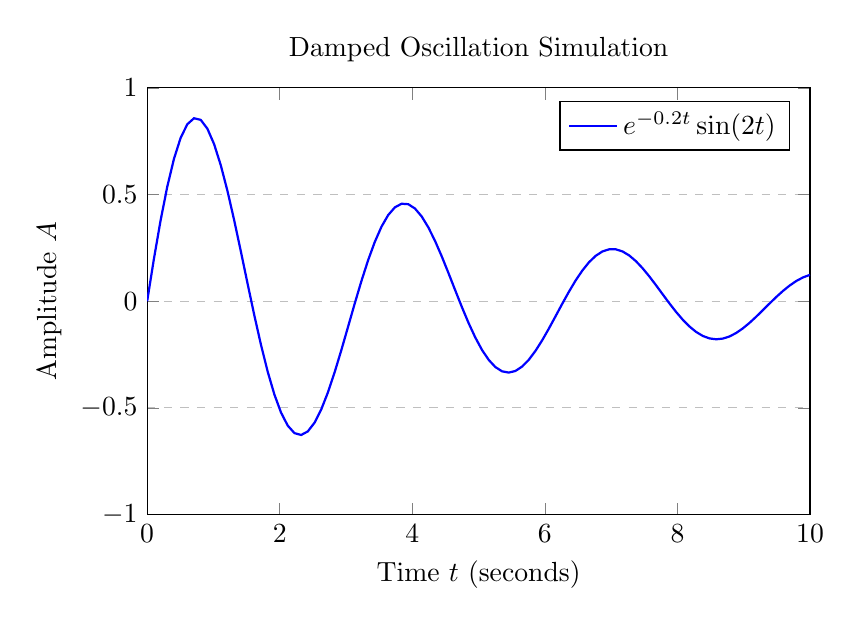
\begin{tikzpicture} % Changed from \begin{text}
\begin{axis}[
    title={Damped Oscillation Simulation},
    xlabel={Time $t$ (seconds)},
    ylabel={Amplitude $A$},
    xmin=0, xmax=10,
    ymin=-1, ymax=1,
    xtick={0,2,4,6,8,10},
    ytick={-1,-0.5,0,0.5,1},
    legend pos=north east,
    ymajorgrids=true,
    grid style=dashed,
    width=10cm, height=7cm
]

\addplot[
    color=blue,
    thick,
    domain=0:10,
    samples=100,
]
{exp(-0.2*x) * sin(deg(2*x))};
\addlegendentry{$e^{-0.2t} \sin(2t)$}

\end{axis}
\end{tikzpicture} % Changed from \end{text}
\end{center}

\end{document}
